\documentclass[12pt, a4paper]{article}

% --- Packages ---
\usepackage[utf8]{inputenc}
\usepackage[T1]{fontenc}
\usepackage[french]{babel}
\usepackage{graphicx}
\usepackage{amsmath}
\usepackage{amssymb}
\usepackage{geometry}
\usepackage{hyperref}
\usepackage{booktabs}
\usepackage{float}
\usepackage{titlesec}
\usepackage{xcolor}
\usepackage{caption}

% --- Mise en page ---
\geometry{top=2.5cm, bottom=2.5cm, left=2.5cm, right=2.5cm}
\hypersetup{
    colorlinks=true,
    linkcolor=blue!70!black,
    urlcolor=blue!70!black,
}

\begin{document}

% ==========================================
%              PAGE DE GARDE
% ==========================================
\begin{titlepage}
    \centering
    
    % --- En-tête avec les logos ---
    \begin{minipage}{0.45\textwidth}
        \begin{flushleft}
            
\includegraphics[width=0.9\textwidth]{fsbm_logo.png}
        \end{flushleft}
    \end{minipage}
    \hfill
    \begin{minipage}{0.45\textwidth}
        \begin{flushright}
            
\includegraphics[width=0.8\textwidth]{DSBD.png}
        \end{flushright}
    \end{minipage}

    \vspace*{2cm}

    % --- Nom de l'université et de la formation ---
    \textsc{\LARGE Université Hassan II de Casablanca}\\[0.5cm]
    \textsc{\Large Faculté des Sciences Ben M'Sick}\\[0.5cm]
    \textsc{\large Master Data Science et Big Data}\\[2cm]

    % --- Titre du rapport ---
    \rule{\linewidth}{0.5mm} \\[0.5cm]
    { \huge \bfseries Analyse Comparative :\\[0.3cm] Métaheuristiques vs Descente de Gradient \\[0.5cm] }
    \rule{\linewidth}{0.5mm} \\[1.5cm]

    % --- Sous-titre ---
    \Large \textit{Application à la classification sur le dataset Iris}\\[3cm]

    % --- Auteur et informations annexes ---
    \begin{minipage}{0.45\textwidth}
        \begin{flushleft} \large
            \emph{Réalisé par :}\\
            \textbf{Achraf Chahid}
        \end{flushleft}
    \end{minipage}
    \hfill
    \begin{minipage}{0.45\textwidth}
        \begin{flushright} \large
            \emph{Année Universitaire :}\\
            \textbf{2025 - 2026}
        \end{flushright}
    \end{minipage}

    \vfill

    % --- Date ---
    {\large \today}
\end{titlepage}

% ==========================================
%              CORPS DU DOCUMENT
% ==========================================
\newpage
\tableofcontents
\newpage

% ---------------------------------------------------------
\section{Introduction}
L'entraînement des réseaux de neurones profonds repose fondamentalement sur la minimisation d'une fonction de perte dans un espace multidimensionnel. Historiquement, les méthodes d'optimisation basées sur le gradient, telles que la descente de gradient stochastique (SGD) et ses variantes adaptatives (Adam), constituent le standard industriel. Elles s'appuient sur la dérivabilité de la fonction objectif pour converger rapidement vers un minimum local.

Cependant, face à des fonctions non lisses, non différentiables, ou des paysages d'optimisation fortement non convexes criblés de minima locaux trompeurs, ces méthodes peuvent échouer. C'est dans ce contexte que les métaheuristiques, inspirées de processus naturels, offrent une alternative robuste. L'optimisation par essaim particulaire (PSO - \textit{Particle Swarm Optimization}) en est un excellent représentant, privilégiant une exploration globale stochastique plutôt qu'une exploitation purement locale.

L'objectif de ce projet est de réaliser une étude empirique comparant rigoureusement SGD, Adam et PSO. Pour éviter la malédiction de la dimensionnalité qui pénalise dramatiquement les méthodes populationnelles comme PSO, l'étude s'appuie sur un problème de complexité maîtrisée : la classification multiclasse du dataset Iris. Afin d'enrichir l'analyse, cette implémentation algorithmique s'accompagne du développement d'une architecture full-stack (API et Interface Web) permettant la simulation visuelle de ces trajectoires d'optimisation.

% ---------------------------------------------------------
\section{Méthodologie et Architecture}

\subsection{Données et Modélisation Mathématique}
Le dataset Iris (150 échantillons, 4 caractéristiques continues, 3 classes cibles) a été partitionné selon un ratio strict de 80/20 pour séparer les ensembles d'apprentissage et de test. Une standardisation (Z-score) a été appliquée en amont pour assurer la stabilité numérique des gradients.

Afin d'isoler véritablement l'impact de l'algorithme d'optimisation sur l'apprentissage, un Perceptron Multicouche (MLP) minimaliste a été modélisé en utilisant le framework PyTorch. L'architecture se définit comme suit :
\begin{itemize}
    \item Une couche d'entrée $X \in \mathbb{R}^{4}$.
    \item Une couche cachée dense composée de 10 neurones, activée par une fonction non linéaire ReLU : $h = \max(0, W_1 X + b_1)$.
    \item Une couche de sortie $Y \in \mathbb{R}^{3}$, dont la perte est évaluée via l'entropie croisée (\textit{Cross-Entropy Loss}).
\end{itemize}
Ce modèle totalise exactement 83 paramètres optimisables (poids et biais). C'est ce vecteur $\theta \in \mathbb{R}^{83}$ que nos optimiseurs devront calibrer.

\subsection{Les Algorithmes Déployés}
\begin{enumerate}
    \item \textbf{Stochastic Gradient Descent (SGD) :} Implémentation classique avec un taux d'apprentissage fixe. Il sert de \textit{baseline} théorique.
    \item \textbf{Adam (Adaptive Moment Estimation) :} Optimiseur de pointe qui calcule des taux d'apprentissage adaptatifs pour chaque paramètre en estimant les moments du premier (moyenne) et second ordre (variance non centrée) des gradients.
    \item \textbf{Particle Swarm Optimization (PSO) :} Une métaheuristique développée "from scratch" en PyTorch. La population a été fixée à 30 particules. Chaque particule $i$ navigue dans l'espace $\mathbb{R}^{83}$ en mettant à jour sa vitesse et sa position selon son meilleur historique personnel et le meilleur historique global de l'essaim, sans jamais calculer la dérivée de la fonction de perte.
\end{enumerate}

\subsection{Architecture Logicielle Découplée (Full-Stack)}
Au-delà du script d'entraînement classique, ce projet s'est distingué par l'intégration d'une architecture logicielle professionnelle, séparant la logique d'optimisation mathématique de sa restitution visuelle.

% --- IMAGE 1 : ARCHITECTURE (OPTIONNELLE) ---
% Si vous avez un schéma draw.io de votre architecture, décommentez la suite :
% \begin{figure}[H]
%     \centering
%     \includegraphics[width=0.75\textwidth]{architecture.png}
%     \caption{Architecture découplée : Moteur d'optimisation backend (FastAPI/PyTorch) et Tableau de bord frontend (React/Plotly)}
%     \label{fig:archi}
% \end{figure}

Le backend a été développé avec \textbf{FastAPI} pour exposer les trajectoires générées par les algorithmes sous forme de service web (API RESTful). Le frontend, construit avec \textbf{React et Tailwind CSS}, consomme ces données de manière asynchrone pour animer les trajectoires sur un tableau de bord analytique.

% ---------------------------------------------------------
\section{Résultats Expérimentaux}

Les trois algorithmes ont été entraînés sur le dataset Iris pendant 100 itérations, dans des conditions matérielles strictement identiques (exécution CPU, initialisation des poids via \textit{seed} fixe).

\subsection{Synthèse des Métriques}

Le tableau \ref{tab:results} expose les performances finales. La dichotomie entre la précision mathématique et le coût computationnel y est évidente.

\begin{table}[H]
    \centering
    \begin{tabular}{lccc}
        \toprule
        \textbf{Optimiseur} & \textbf{Temps d'exécution (s)} & \textbf{Perte Finale (Train)} & \textbf{Précision (Test)} \\
        \midrule
        \textbf{SGD} & 0.179 & 0.94100 & 70.0\% \\
        \textbf{Adam} & \textbf{0.155} & 0.08361 & \textbf{100.0\%} \\
        \textbf{PSO} & 0.425 & \textbf{0.03781} & \textbf{100.0\%} \\
        \bottomrule
    \end{tabular}
    \caption{Comparaison empirique de la qualité de la solution et du coût computationnel}
    \label{tab:results}
\end{table}

\subsection{Analyse Cinétique de la Convergence}

Pour comprendre ces métriques, l'observation des courbes de convergence est primordiale.

% --- IMAGE 2 : COURBE DE CONVERGENCE ---
\begin{figure}[H]
    \centering
    % Remplacez 'convergence.png' par le nom exact de votre fichier
    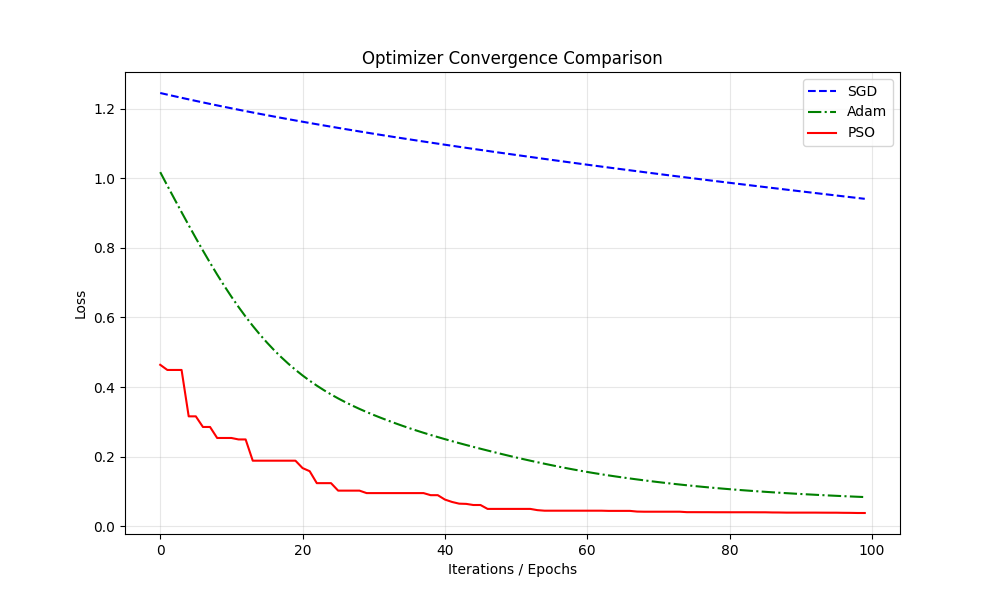
\includegraphics[width=0.85\textwidth]{convergence.png}
    \caption{Évolution de la fonction de perte (Cross-Entropy) au fil des itérations}
    \label{fig:convergence}
\end{figure}

L'analyse de la figure \ref{fig:convergence} révèle trois comportements structurellement différents :
\begin{itemize}
    \item \textbf{La rigidité de SGD :} Avec un pas d'apprentissage fixe de $0.01$, SGD peine à descendre efficacement le long des ravins de la fonction de perte. En 100 itérations, il n'atteint qu'une précision médiocre (70\%).
    \item \textbf{La fulgurance d'Adam :} Grâce à sa capacité à accumuler de l'inertie (Momentum) et à moduler son apprentissage, Adam descend la surface d'erreur avec une fluidité remarquable, atteignant rapidement un excellent minimum local.
    \item \textbf{L'exploration en paliers de PSO :} La courbe rouge de PSO démontre la nature stochastique de l'algorithme. La fonction de perte stagne pendant que l'essaim explore, puis chute brutalement lorsqu'une particule découvre une meilleure région. In fine, PSO trouve un minimum global \textbf{plus bas que celui d'Adam} (0.037 vs 0.083).
\end{itemize}

% ---------------------------------------------------------
\section{Simulation Avancée et Limites Analytiques}

\subsection{Visualisation des Trajectoires sur la Fonction de Rastrigin}
Pour pallier l'impossibilité de visualiser l'espace en 83 dimensions du modèle Iris, nous avons conçu un outil de simulation web. L'API projette les algorithmes sur la \textbf{fonction de Rastrigin en 2D}, une surface mathématique délibérément criblée de minima locaux pièges.

% --- IMAGE 3 : DASHBOARD WEB ---
\begin{figure}[H]
    \centering
    % Remplacez 'dashboard_ui.png' par la capture d'écran de votre interface web
    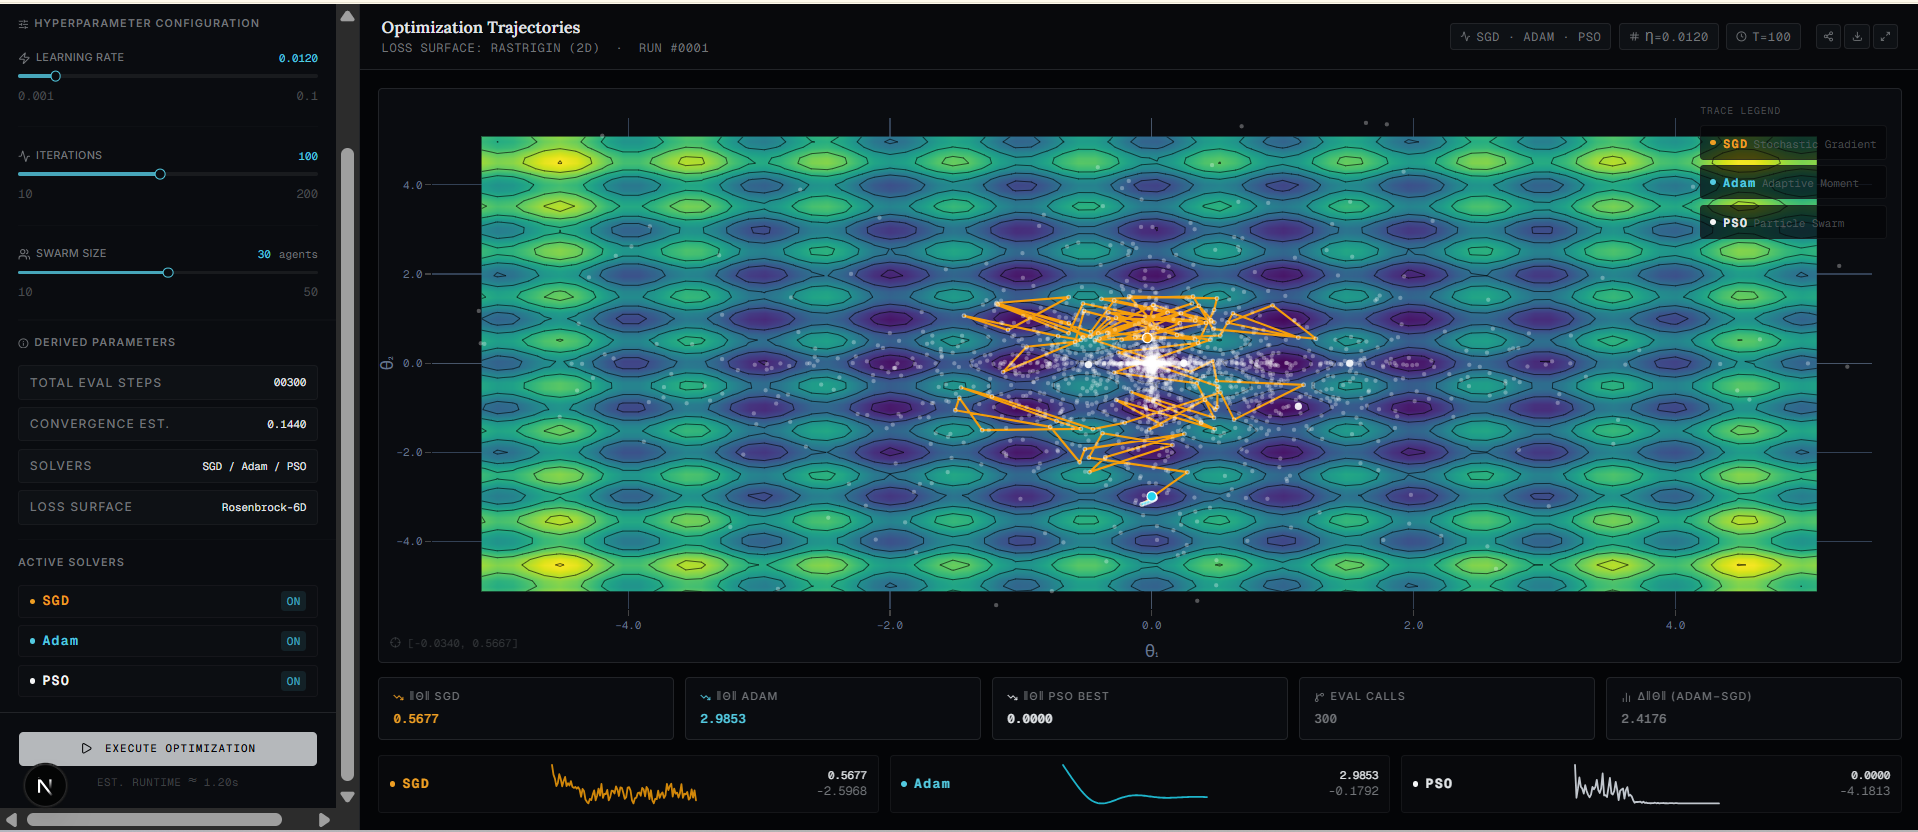
\includegraphics[width=0.95\textwidth]{dashboard_ui.png}
    \caption{Tableau de bord interactif (React/Plotly) illustrant l'évitement des minima locaux}
    \label{fig:dashboard}
\end{figure}

Comme l'illustre l'interface analytique (Figure \ref{fig:dashboard}), les méthodes de gradient strict (SGD, Adam) ont une forte propension à converger vers le minimum local le plus proche de leur point d'initialisation. À l'inverse, l'essaim particulaire (PSO) disperse ses agents. Si certaines particules sont piégées, elles sont finalement "rappelées" par l'influence gravitationnelle de la particule ayant découvert le véritable minimum global.

\subsection{La Limite Inhérente : Le Passage à l'Échelle (Scalability)}
Si PSO triomphe sur la qualité de la solution finale dans un espace restreint ($\mathbb{R}^{83}$), le tableau \ref{tab:results} trahit sa principale faiblesse : le temps de calcul. PSO nécessite ici $0.425$ secondes contre $0.155$ secondes pour Adam. 

Dans un algorithme de gradient, chaque lot de données (batch) ne requiert qu'une seule passe aller-retour (Forward/Backward propagation) pour ajuster le modèle complet. Pour PSO, sans calcul de gradient, le modèle doit évaluer la fonction de perte par \textit{Forward pass} complète pour \textbf{chaque particule} à \textbf{chaque itération}. Sur un réseau de grande envergure (ex: ResNet, Transformers avec des millions de paramètres), l'espace de recherche devient trop vaste. L'exploration stochastique par essaim subit la "malédiction de la dimensionnalité", rendant la convergence non seulement atrocement lente, mais souvent impossible.

% ---------------------------------------------------------
\section{Conclusion}

Ce projet d'ingénierie appliquée confirme qu'en matière d'optimisation mathématique pour le Machine Learning, la loi du "No Free Lunch" prévaut. 

\begin{itemize}
    \item Les \textbf{méthodes basées sur le gradient}, notamment les variantes adaptatives comme Adam, sont indispensables à l'ère du Deep Learning. Leur rapport coût-calcul/efficacité est imbattable sur des fonctions différentiables de très grande dimension.
    \item Les \textbf{métaheuristiques populationnelles}, comme PSO, offrent une résilience fascinante face aux surfaces non convexes et non dérivables. Bien qu'inadaptées à l'entraînement direct des poids de grands réseaux de neurones, elles restent des outils redoutables pour des tâches d'exploration complexe, comme l'optimisation des hyperparamètres (Hyperparameter Tuning) ou la conception d'architecture neuronale (Neural Architecture Search).
\end{itemize}

Enfin, le déploiement de ces mécanismes d'optimisation au sein d'une architecture applicative distribuée (FastAPI / React) a démontré l'importance cruciale de coupler la rigueur des Data Sciences aux bonnes pratiques du Software Engineering (Data Engineering) pour rendre les modèles explicables et accessibles.

\end{document}